\section{Analysing play in video}
\subsection{Theory}
The video analysis is built more specifically for the video provided. The ball in the video never changes and lighting in the video is pretty good. We are able to convert each frame into HSL colour space and highlighting light and nearly white objects based on a range. This is then able to generate a mask with the ball, and some other lines or artifacts from the players. A grayscale image of each frame is then compared with the frame before it to find any changes, this difference is then thresholded to allow us to combine the HSV mask with the difference mask to find just the ball. Next, the position and the direction of travel of the ball are taken into account. The position is determined from the contours of the mask binary image produced from the previously mentioned steps. This position is then added to an array so that the direction of the ball can be considered. Any change in direction suggests how the ball as bounced, if a ball goes down and up it has bounced off the table, if the ball bounces right to left Player 1 has hit the ball, if the ball bounces left to right, player 2 has hit the ball. A bounding box around the net has been created to handle hits to the net. The bounding box does not include the full net because this may trigger false positives when the ball flies over the far side of the net. 
\subsection{Results \& Illustrations}
See below the video and data streaming.
\begin{figure}[H]
    \centering
    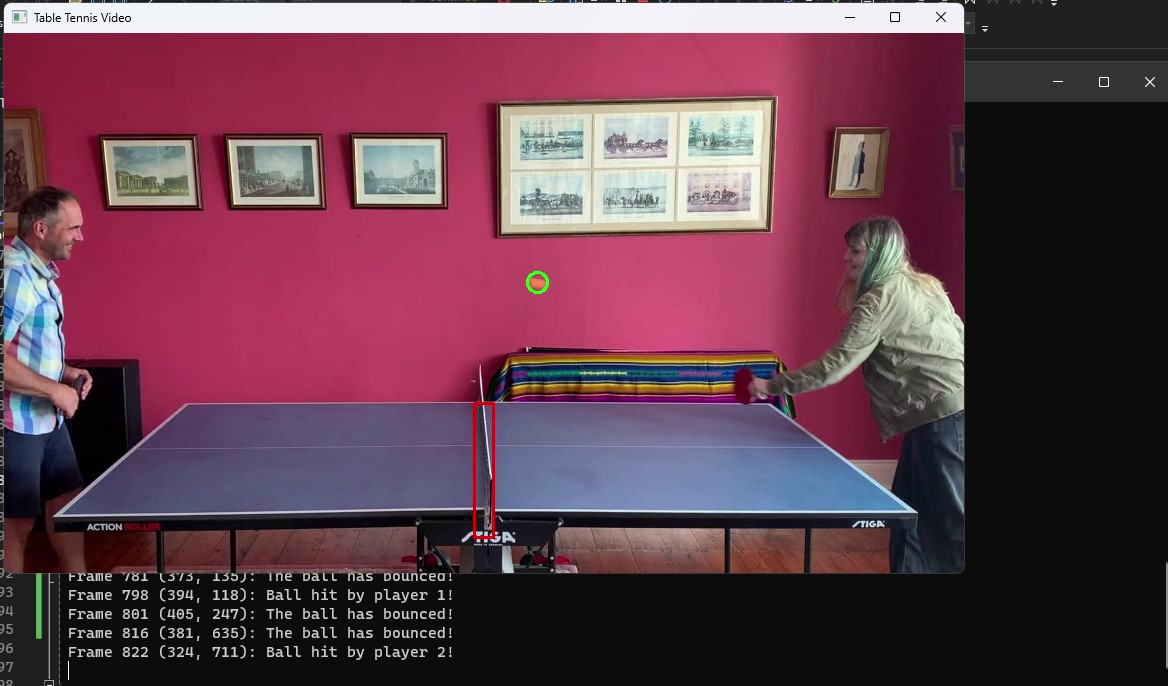
\includegraphics[width=0.75\textwidth]{results/frame.jpg}
    \caption{\href{https://youtu.be/y1nezl333-0}{Run through of Video Analysis}\href{https://youtu.be/y1nezl333-0}{https://youtu.be/y1nezl333-0}}
    \label{fig:vid-anyl}
\end{figure}

\subsection{Analysis}
There are some issues when a player first serves the ball. Due to the unexpected change in direction, hits are recorded sooner than they take place. Given more time, some more logic could be added to more accurately determine the hits off the net.